\documentclass[11pt]{article}

% Links
\usepackage{hyperref}
\makeatletter
\g@addto@macro{\UrlBreaks}{\UrlOrds}
\makeatother

% Margins
\usepackage[left=20mm, bottom=30mm,right=20mm]{geometry}

% Maths
\usepackage{siunitx}
\usepackage{amsmath}

% Code
\usepackage{listings}
\definecolor{codegreen}{rgb}{0,0.6,0}
\definecolor{codegray}{rgb}{0.5,0.5,0.5}
\definecolor{codepurple}{rgb}{0.58,0,0.82}
\definecolor{backcolour}{rgb}{0.95,0.95,0.92}
\lstdefinestyle{mystyle}{
    backgroundcolor=\color{backcolour},   
    commentstyle=\color{codegreen},
    keywordstyle=\color{magenta},
    numberstyle=\tiny\color{codegray},
    stringstyle=\color{codepurple},
    basicstyle=\ttfamily\footnotesize,
    breakatwhitespace=false,         
    breaklines=true,                 
    captionpos=b,                    
    keepspaces=true,                 
    numbers=left,                    
    numbersep=5pt,                  
    showspaces=false,                
    showstringspaces=false,
    showtabs=false,                  
    tabsize=2
}
\lstset{style=mystyle}


% Underlines
\usepackage{ulem}

% Imports
\usepackage{import}

% Graphics
\usepackage{graphicx}

% Plots
\usepackage{pgfplots}
\pgfplotsset{width=10cm,compat=1.9}

% Picture for title
\usepackage[demo]{graphicx}
\usepackage{subcaption}
\usepackage{titlepic}

% Language 
% \usepackage[english]{babel}

% Headers and footers
\usepackage{fancyhdr}
\pagestyle{fancyplain}
\fancyhf{}
\lhead{\fancyplain{}{Redes de Computadores - 1º Trabalho Laboratorial}}
\lfoot{\fancyplain{}{}}
\cfoot{\thepage}

% Paragraph indentation
\usepackage{indentfirst}

% Picture
\titlepic{\begin{figure}[t!]
\centering
\subfloat{{
\includegraphics[width=7cm]{img/unnamed.png} }}%
\qquad
\subfloat{{
\includegraphics[width=7cm]{img/Cienciasporto.png} }}%
%\vspace{-3.0cm}
\end{figure}}
% Date
\date{Dezembro, 2021}
% Title
\title{\Huge{\textbf{Protocolo de Ligação de Dados \\
\Large{ Redes de Computadores - 1º Trabalho Laboratorial }}}}
% Author
\author{
\textbf{\Large Class 9 group 2} \vspace{0.5em} \\
\begin{tabular}{r l}
	\email{up201906086@edu.fe.up.pt} & Marcelo Henriques Couto \\
	\email{up201907361@edu.fe.up.pt} & Francisco Pinto de Oliveira \\
\end{tabular}
}

% No paragraph indentation
% \parindent=0pt

% Start the document
\begin{document}
\maketitle

\newpage
\tableofcontents

\newpage
\section{Sumário}

Este relatório tem pretende descrever a implementação do 1º trabalho laboratorial de Redes de Computadores, expondo detalhes de funcionamento, implementação e eficiência.

O trabalho foi concluído com sucesso e a aplicação é capaz de transmitir ficheiros utilizando a porta série.


\section{Introdução}

O trabalho desenvolvido teve como objetivo desenvolver um protocolo de transmissão de dados através da porta série. Este relatório pretende descrever o funcionamento e detalhes de implementação.

O relatório será organizado nos seguintes módulos:
\begin{itemize}
    \item \textbf{Arquitetura} – blocos funcionais e interfaces
    \item \textbf{Estrutura do código} – principais funções e estruturas de dados bem como a sua relação com a arquitetura
    \item \textbf{Casos de uso} – identificação e sequencia de chamada de funções
    \item \textbf{Protocolo de ligação lógica} – descrição de funcionamento do protocolo e exemplificação apresentando fragmentos de código
    \item \textbf{Protocolo da aplicação} – descrição do funcionamento da camada e exemplificação apresentando fragmento de código
    \item \textbf{Validação} – descrição dos testes efetuados
    \item \textbf{Eficiência do protocolo de ligação de dados} – caracterização da eficiência do protocolo de ligação de dados
    \item \textbf{Conclusões} – síntese da informação apresentada nas secções anteriores e reflexão sobre objetivos e aprendizagens
\end{itemize}
    

\section{Arquitetura}
Em termos de arquitetura a aplicação está dividida em \textbf{três camadas}: \textbf{aplicação}, \textbf{ligação de dados} e \textbf{protocolo}. Para além disso, ainda há \textbf{dois modos de funcionamento}: \textbf{emissor e recetor}. As camadas traduzem-se em módulos de código, mas os modos de funcionamento não. Isto acontece porque o utilizador utiliza o mesmo executável tanto para o emissor quanto para o recetor e o utilizador escolhe o modo de funcionamento utilizando argumentos de linha de comandos. 

\begin{figure}[h!]
    \centering
    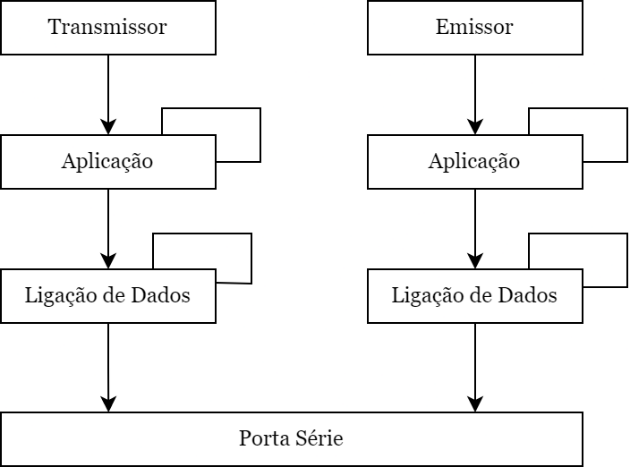
\includegraphics[width=10cm]{img/pic.png}    
    \caption{Arquitetura da aplicação}
\end{figure}

\begin{itemize}
    \item A \textbf{camada da aplicação} é a responsável leitura/criação do novo ficheiro. O comportamento desta camada tem de ser especificado para determinar o seu comportamento
    \item A \textbf{camada de ligação de dados} é a responsável tanto por ler e escrever na porta série quanto por lidar com possíveis erros na transmissão das tramas. Esta camada não tem qualquer autonomia, só realiza as ações de transmissão e emissão quando solicitada
    \item A \textbf{camada de protocolo} já está implementada e a interação é feita através de system calls
\end{itemize}


\section{Casos de Uso Principais}

\subsection{Identificação}

Para utilizar o programa o utilizador deve compilá-lo. Para isso deve executar o comando "make". Se o código já tiver sido previamente compilado deve ser executado "make clean".

Para transmitir um ficheiro o utilizador deve possuir dois terminais ligados por uma porta série.
\begin{itemize}
    \item Comando a executar no terminal do transmissor - ./rcompy -t -s \textit{caminho para a porta série} -f \textit{caminho para o ficheiro}
    \item Comando a executar no terminal do recetor - ./rcompy -r -s \textit{caminho para a porta série} -f \textit{caminho para o novo ficheiro}
    \item Opções extra como -x \textit{frequência de erros nos dados} ou -z \textit{frequência de erros no cabeçalho} e -p \textit{tempo de propagação} podem ser acrescentadas ao recetor para simulação de erros e tempo de propagação
    \item Para transmitir um ficheiro o utilizador deve possuir dois terminais ligados por uma porta série. 
\end{itemize}



\subsection{Sequência de Chamadas}

A sequência de chamada a funções de cada componente da aplicação é apresentada nos seguintes diagramas.

\begin{figure}[h!]
    \centering
    \begin{subfigure}{.5\textwidth}
        \centering
        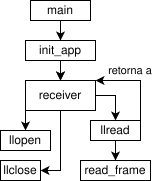
\includegraphics[width=.5\linewidth]{img/EsquemaChamadaAFuncoesReceiver.png}
        \caption{Esquema de Chamadas do Recetor}
    \end{subfigure}%
    \begin{subfigure}{.5\textwidth}
        \centering
        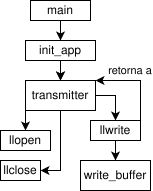
\includegraphics[width=.5\linewidth]{img/EsquemaChamadaAFuncoesTransmiter.png}
        \caption{Esquema de Chamadas do Transmissor}
    \end{subfigure}
    \caption{Esquema de Chamadas do Programa}
\end{figure}

Apenas foram apresentadas as funções mais importantes, o fluxo completo pode ser obtido analisando o código e os seus comentários.




\section{Protocolo de Ligação Lógica}

Os objetivos principais da camada de ligação de dados são:

\begin{enumerate}
    \item Redução e controlo dos erros de transmissão
    \item Regulação do fluxo de dados
    \item Disponibilização de uma interface para comunicação através da porta série à camada de aplicação
\end{enumerate}



\subsection{Leitura da Porta Série}

Para leitura da porta série adaptada da máquina de estados fornecida, para suportar frames de dados, e tem como intuito ler as tramas recebidas na porta e verificar a sua validade. 

A máquina de estados lê dados da porta série byte a byte. Depois da receção do BCC1, se não for detetada uma FLAG, sabemos que estamos perante uma frame de informação. Os dados são colocados num buffer e a leitura acaba quando é encontrada uma FLAG. O buffer contém os dados até à posição N - 1 pois o dado de posição N é o BCC2. Em seguida apresenta-se a sua implementação em pseudocódigo.  

\begin{lstlisting}[caption=Pseudocódigo da StateMachine]
    buffer <- Empty
    While state != STOP:
        byte_rcvd <- read_from_serial_port
        if (state == START) then:
            if byte_rcvd == FLAG then:
                state <- FLAG_RCVD
        if (state == FLAG_RCVD):
            if (isA(byte_rcvd)) then:
                state <- A_RCVD
        if (state == A_RCVD) then:
            if (isC(byte_rcvd)) then:
                state <- A_RCVD
            ElseIf (byte_rcvd == FLAG) then:
                state = FLAG_RCVD
            Else:
                state = START
        if (state == C_RCVD) then:
            if (validBCC1()) then:
                state = BCC_OK
            ElseIf (byte_rcvd == FLAG) then:
                state = FLAG_RCVD
            Else:
                state = START
        if (state == BCC_OK) then:
            if (byte_rcvd == FLAG_RCVD) then:
                state <- STOP
            Else:
                Insert(buffer, byte_rcvd)
                state = DATA
        if (state == DATA) then:
            if (byte_rcvd == FLAG) then:
                state = STOP
            Else:
                Insert(buffer, byte_rcvd)
\end{lstlisting}

Quando a verificação do BCC1 falha não se envia qualquer resposta uma vez que é impossível determinar o tipo de frame recebido.

Cada frame é lido num loop para o caso de haver erros na parte de informação e ser necessário receber outro frame. Se o BCC2 for válido e o frame corresponder ao número esperado um RR é enviado senão é enviado REJ e aguarda-se pelo novo frame.

\begin{lstlisting}[language=C, caption=Código em C do loop responsével pela leitura da porta série, em llread]
while(!valid_frame) {
    new_frame = read_frame(fd, link_layer_data.frame, MAX_FRAME_SIZE);
    frame_size = destuff(link_layer_data.frame, new_frame.packet_size, aux_buffer, MAX_PACKET_SIZE + 1);

    if (frame_size == 0) {
        fprintf(stderr, "Error in data_link - llread: destuffing packet unsuccessfull\n");
        return -1;
    }
    uint8_t bcc2 = aux_buffer[--frame_size];

    // Error
    if (new_frame.frame_type != expected_package || !validBCC2(bcc2, aux_buffer, frame_size)) {
        if (assemble_supervision_frame(expected_package ? REJ_1 : REJ_0, RECEIVER, response_frame) == -1) return -1;
    } else {
        memcpy(buffer, aux_buffer, frame_size);
        if (assemble_supervision_frame(expected_package ? RR_0 : RR_1, RECEIVER, response_frame) == -1) return -1;
        valid_frame = true;
    }
    if (write(fd, response_frame, SUPV_FRAME_SIZE) != 5) {
        fprintf(stderr, "Error in data_link - llread: did not write response frame correctly");
        return -1;
    }
}
\end{lstlisting}

\subsection{Escrita na Porta Série}

Quando um buffer é escrito, o utilizador da função deve especificar uma resposta esperada pelo outro lado da porta série. Quando o buffer é enviado, é acionado um alarme. Se o alarme for chamado uma flag é ativada e retira-se um valor ao número de tentativas de leitura. Se o número de tentativas for esgotado, assume-se que a trama não foi enviada.
\begin{lstlisting}[language=C, caption=Código em C da função responsável pela escrita na porta série]
/* Writes a buffer to the serial port and awaits a certain response
    fd -> Serial port file desciptor
    buffer -> buffer to write
    length -> length of the buffer to be written
    expected_response -> expected response sent by the other end of the serial port
*/
int write_buffer(int fd, uint8_t* buffer, size_t length, FrameType expected_response) 
\end{lstlisting}

\subsection{Interface para uso na camada de aplicação}

O programa foi desenhado de modo a manter independência entre a camada de aplicação e o protocolo de ligação de dados, de modo que este último é apenas visível à camada superior como 4 pontos de entrada.

\subsubsection{Estabelecimento da ligação}

Para o estabelecimento de ligação através de uma porta série, a função disponibilizada \textbf{llopen}. 

\begin{itemize}
    \item Emissor - configura-se a porta série, envia-se uma trama \textbf{SET} (pelo emissor) e aguarda-se uma trama \textbf{UA} que será enviada pelo recetor
    \item Recetor - configura-se a porta série, aguarda-se a receção de uma trama \textbf{SET}; quando esta é recebida corretamente, envia-se uma trama \textbf{UA} de modo a marcar o estabelecimento de ligação
\end{itemize}

\begin{lstlisting}[language=C, caption=llopen header]
int llopen(char* port, ConnectionType role)
\end{lstlisting}

\subsubsection{Término da conexão}

Para o fecho da ligação, o protocolo de ligação de dados fornece a função \textbf{llclose}.

\begin{itemize}
    \item Emissor - envia-se uma trama \textbf{DISC}, aguarda-se por uma trama \textbf{DISC} e finalmente envia-se uma trama \textbf{UA}.
    \item Recetor - aguarda-se uma trama \textbf{DISC}, envia-se uma trama \textbf{DISC} e finalmente aguarda-se uma trama \textbf{UA}.
\end{itemize}


\begin{lstlisting}[language=C, caption=llclose header]
int llclose(int fd)
\end{lstlisting}


\subsubsection{Envio de dados}

Para o envio de dados (pela parte do emissor), existe a função \textbf{llwrite}.

Esta função apenas invoca a função \texttt{write\_buffer} descrita acima, além de controlar o número de sequência da trama.

\subsubsection{Receção de dados}

Para a receção de dados (pela parte do recetor), é providenciada a função \textbf{llread}.

Esta função invoca a \texttt{state\_machine} e controla o processo de deteção de erros descritos acima.

\section{Protocolo de Aplicação}

O Protocolo de Aplicação implementado tem como objetivos:
\begin{enumerate}
    \item Envio, receção e construção dos pacotes de controlo de início e fim de transmissão
    \item Leitura/Escrita de dados de/para uma porta série utilizando o protocolo de ligação lógica
    \item Construção/Interpretação de pacotes de dados com \textit{headers} válidos
    \item Divisão de um ficheiro em fragmentos e posterior envio (transmissor)
    \item Construção de um ficheiro através de dados recebidos (recetor)
\end{enumerate}


\subsection{Pacotes de Controlo}

Os pacotes de controlo de transmissão são construídos pelo transmissor para denotar o inicio e fim de transmissão, bem como o envio de informação sobre os dados a serem enviados, tal como o tamanho do ficheiro e o seu nome. 

\begin{lstlisting}[language=C, caption=Função que constrói o pacote de controlo (transmissor)]
uint8_t* build_control_packet(size_t* control_packet_size, char* file_name) 
\end{lstlisting}

\begin{lstlisting}[language=C, caption=Função que interpreta o pacote de controlo recebido (recetor)]
void parse_control_packet(uint8_t* packet) 
\end{lstlisting}

O tamanho do ficheiro, enviado no inicio da ligação no pacote de controlo, é usado para verificar, no fim da ligação, se o número de bytes recebidos corresponde ao esperado.

\begin{lstlisting}[language=C, caption=Verificação do tamanho do ficheiro recebido (receiver)]
    if (bytes_received != app_data.transfer_file_size) {
        fprintf(stderr, "File size does not correspond to the expected\n");
    }
\end{lstlisting}

\subsection{Leitura e Escrita de dados}

A leitura e escrita de dados são ambos efetuados em loops nas funções principais do emissor e recetor, \textbf{transmitter} e \textbf{receiver} respetivamente.

\begin{lstlisting}[language=C, caption=Envio de pacotes de dados]
while (bytes_read < app_data.transfer_file_size) {
    packet_no++;
    bytes_written = read_data_packet(packet_no, data_packet, oldFileDescriptor, bytes_read);
    bytes_read += bytes_written - 4;
    if ((llwrite(app_data.file_descriptor, data_packet, bytes_written)) == -1) exit(1);
    printf("Transmitter - packet %d sent\n", packet_no);
}
\end{lstlisting}


\begin{lstlisting}[language=C, caption=Leitura dos pacotes de dados]
    while (true) {
        // READ
        if (llread(app_data.file_descriptor, data_packet, MAX_PACKET_SIZE) == -1) exit(1);
        if (data_packet[0] == 0x01) {
            bytes_received += write_data_packet(data_packet, newFileDescriptor, &packet_no);
            printf("Receiver - packet %d received\n", (int) data_packet[1]);
        } else if (data_packet[0] == 0x02) {
            parse_control_packet(data_packet);
            if (file_exists(app_data.transfer_file_dir, app_data.transfer_file_name)) {
                fprintf(stderr, "Error in application - receiver: file already exists\n");
                exit(1);
            }
            newFileDescriptor = open_transfer_file();
            fileOpen = true;

        } else if (data_packet[0] == 0x03) {
            // CLOSE
            if ((llclose(app_data.file_descriptor)) != 0) exit(1);
            printf("Receiver - connection cut\n");
            break;
        } else {
            fprintf(stderr, "Error in application - receiver: C byte value invalid\n");
            exit(1);
        }
    }
\end{lstlisting}

Nos pacotes de dados possuem numeração, que permitem avisar qualquer inconsitência nos pacotes recebidos. Esta verificação é feita na função \texttt{read\_data\_packet}. \textbf{Nota:} esta funcionalidade foi implementada posteriormente à apresentação.
    
\subsection{Leitura do ficheiro e construção dos pacotes}

A leitura do ficheiro do \textbf{emissor} e subsequente construção do pacote de dados é feita incrementalmente, sendo a seguinte função chamada no loop de escrita referido anteriormente.

\begin{lstlisting}[language=C, caption=Função que lê o ficheiro e constrói o pacote de dados]
    size_t read_data_packet(int packetNo, uint8_t* data_packet, int fd, int bytes_read)
\end{lstlisting}

\subsection{Interpretação dos pacotes e escrita do ficheiro}

O \textbf{recetor} executa a interpretação e verificação dos dados recebidos e a escrita dos mesmos num ficheiro numa mesma função, chamada iterativamente no loop acima descrito.

\begin{lstlisting}[language=C, caption=Função que interpreta o pacote de dados recebido e escreve no ficheiro]
    size_t write_data_packet(uint8_t* data_packet, int fd, int* packet_no)
\end{lstlisting}


\section{Validação}

De forma a testar a aplicação e o protocolo desenvolvidos, foram executados os seguintes testes:

\begin{itemize}
    \item Envio de ficheiros de diferentes tamanhos
    \item Interrupção da ligação por cabo entre as portas série
    \item Geração de ruído na ligação através de um curto circuito
    \item Interrupção momentânea da ligação a meio de um envio
    \item Envio de ficheiros com diferentes percentagens de erros simulados
    \item Variação dos tempos de propagação simulados
    \item Envio de ficheiros com diferentes tamanhos das tramas de Informação
    \item Envio de ficheiros para diferentes valores de capacidade de ligação (Baudrate)
\end{itemize}

O sucesso destes testes permitiu-nos concluir que o protocolo e a aplicação funcionam como esperado.

\section{Eficiência}

\subsection{Protocolo utilizado}

O protocolo implementado baseia-se num sistema \textit{Stop-and-Wait ARQ}. O seu nome advém da natureza do comportamento do emissor e do recetor:
\begin{itemize}
    \item \textbf{Stop-and-Wait} porque o emissor espera pela resposta do recetor a cada trama
    \item \textbf{ARQ ou Automatic Repeat Request} porque o recetor automaticamente requer a repetição do envio da trama se esta contiver erros ou não corresponder ao esperado
\end{itemize}

\subsubsection{Funcionamento do protocolo}

\begin{enumerate}
    \item O emissor envia uma trama e espera pela resposta do recetor
    \item \begin{itemize}
        \item Se o recetor receber a trama que espera, envia uma mensagem de acknowledgement ao emissor 'ACK'
        \item Caso receba uma trama que não corresponde à esperada ou que contenha erros,  envia uma mensagem de rejeição, de modo a que o emissor reenvie a mensagem 'NACK'
    \end{itemize}
    \item \begin{itemize}
        \item Recomeça o processo para a próxima trama ou
        \item Reenvia a trama 
    \end{itemize}
\end{enumerate}

\subsubsection{Mecanismos de deteção de erros}

\paragraph{Através da numeração das tramas} com os valores 0 ou 1, o recetor é capaz de distinguir se a trama recebida é aquela que se pretende ou se é apenas uma retransmissão ou se houve um lapso da trama.

\paragraph{BCC1 e BCC2} são dois componentes da trama cuja função é detetar um eventual bit flip no cabeçalho ou conteúdo da trama, respetivamente.

\subsection{Análise de Dados}

De modo a entender de que forma afetam a performance do protocolo alguns dos seus parâmetros, foi executada uma recolha e análise de dados.

O nosso protocolo baseia-se num sistema \textit{Stop-and-Wait ARQ}. 

\subsubsection{Definições}
\paragraph{Descrições}
\begin{itemize}
    \item \textbf{S} - eficiência
    \item \textbf{FER} ou $\boldsymbol{p_e}$ - probabilidade de erro numa trama
    \item \textbf{R} ou $\boldsymbol{T_f}$ - débito recebido
    \item $\boldsymbol{T_prop}$ - tempo de propagação da trama
\end{itemize}

\paragraph{Formulas}
\begin{itemize}
    \item $\boldsymbol{a} = \frac{T_prop}{T_f}$
    \item \textbf{Sem erros:} $\boldsymbol{S} = \frac{T_f}{T_prop + T_f + T_prop} = \frac{1}{2a}$
    \item \textbf{Com erros:} $\boldsymbol{S} = \frac{1 - p_e}{2a}$
\end{itemize}


\subsubsection{Gráficos}

Para a recolha de dados, os valores por defeito são:

\begin{itemize}
    \item $Baudrate = 38400$
    \item $Framesize = 150 B$
    \item $T_prop = 0$
    \item $FER = 0$
\end{itemize}

\paragraph{FER}

Os resultados da nossa análise indicam-nos que as fórmulas a cima descritas, no que toca à influência dos erros na trama na eficiência do protocolo, estão corretos. Estas conclusões são suportadas pelo gráfico abaixo.

\begin{center}
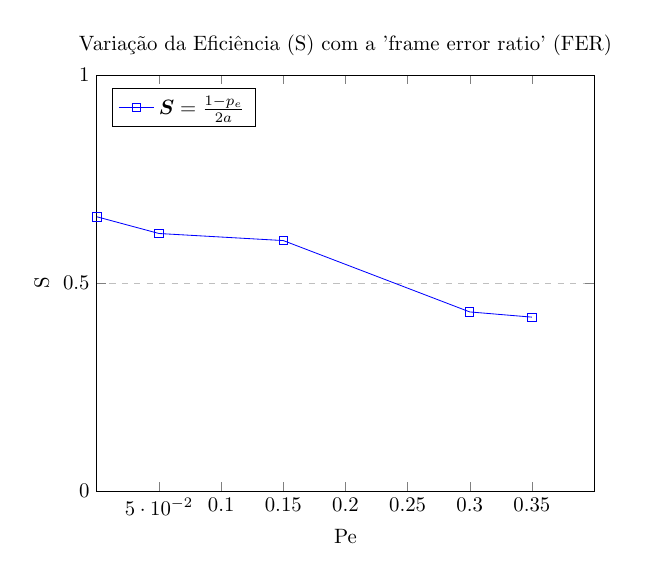
\begin{tikzpicture}[scale = 0.75]
    \begin{axis}[
        title={Variação da Eficiência (S) com a 'frame error ratio' (FER)},
        xlabel={Pe},
        ylabel={S},
        xmin=0, xmax=0.4,
        ymin=0, ymax=1,
        xtick={0.05,0.1,0.15,0.20,0.25,0.30,0.35},
        ytick={0,0.5,1,1.5,2,2.5,3},
        legend pos=north west,
        ymajorgrids=true,
        grid style=dashed,
    ]
    
    \addplot[
        color=blue,
        mark=square,
        ]
        coordinates {
        (0,0.659451659)(0.05,0.619241192)(0.15,0.602266737)(0.30,0.43072573)(0.35,0.418191801)
        };
        \legend{$\boldsymbol{S} = \frac{1 - p_e}{2a}$}
    \end{axis}
    
\end{tikzpicture}
\end{center}

Como a regressão dos dados formou uma função linear, estes vão de encontro à fórmula prevista. A linearidade da função não é muito definida devido ao curto tamanho da amostra, que foi recolhida em laboratório em tempo limitado.


\paragraph{Tempo de propagação}

O próximo gráfico mostra a variação da eficiência consoante o tempo de propagação, o que valida as fórmulas no sentido de que S varia em proporcionalidade inversa com a.
\begin{center}
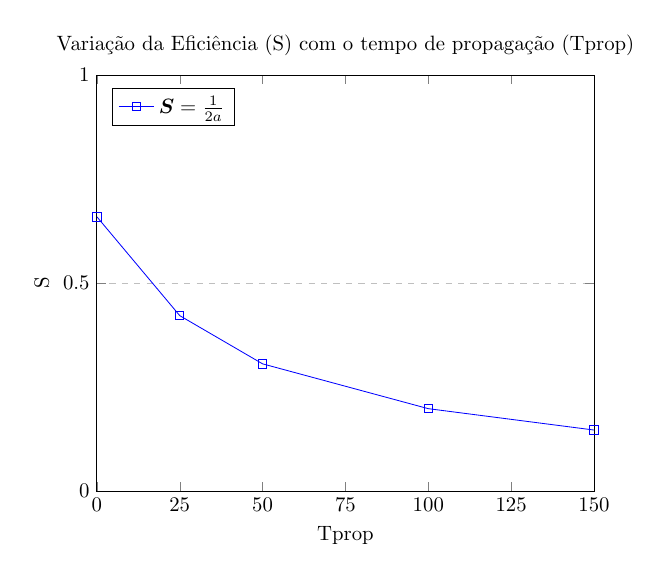
\begin{tikzpicture}[scale = 0.75]
    \begin{axis}[
        title={Variação da Eficiência (S) com o tempo de propagação (Tprop)},
        xlabel={Tprop},
        ylabel={S},
        xmin=0, xmax=150,
        ymin=0, ymax=1,
        xtick={0,25,50,75,100,125,150},
        ytick={0,0.5,1,1.5,2,2.5,3},
        legend pos=north west,
        ymajorgrids=true,
        grid style=dashed,
    ]
    
    \addplot[
        color=blue,
        mark=square,
        ]
        coordinates {
        (0,0.659451659)(25,0.421820196)(50,0.305890228)(100,0.198144294)(150,0.146784865)
        };
        \legend{$\boldsymbol{S} = \frac{1}{2a}$}
    \end{axis}
    
\end{tikzpicture}
\end{center}

\paragraph{Baudrate}

\begin{center}
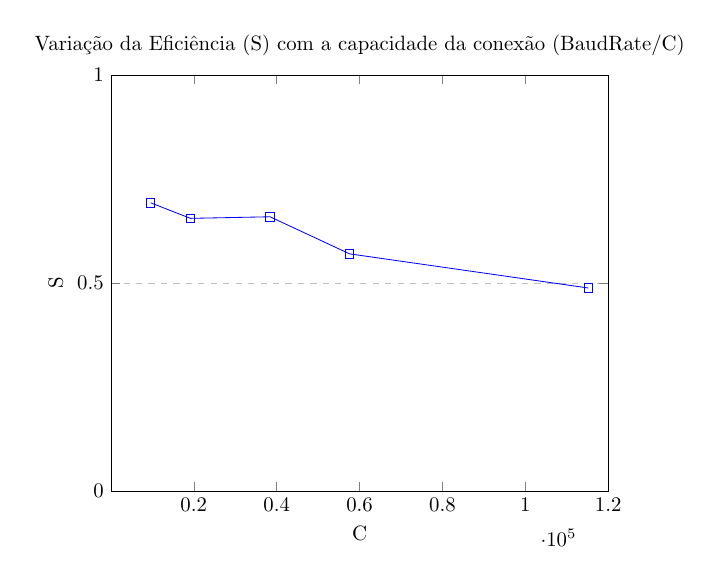
\begin{tikzpicture}[scale = 0.75]
    \begin{axis}[
        title={Variação da Eficiência (S) com a capacidade da conexão (BaudRate/C)},
        xlabel={C},
        ylabel={S},
        xmin=50, xmax=120000,
        ymin=0, ymax=1,
        xtick={0,20000,40000,60000,80000,100000,120000},
        ytick={0,0.5,1,1.5,2,2.5,3},
        legend pos=north west,
        ymajorgrids=true,
        grid style=dashed,
    ]
    
    \addplot[
        color=blue,
        mark=square,
        ]
        coordinates {
        (9600,0.693106848)(19200,0.655667145)(38400,0.659451659)(57600,0.570323225)(115200,0.488247863)
        };
        
    \end{axis}
    
\end{tikzpicture}
\end{center}

O gráfico permite-nos concluir que a eficiência do protocolo diminui com o aumento da capacidade da ligação de dados. Estima-se que esta viesse a subir até um dado valor. No entanto, infelizmente, essa subida não está representada na gama de valores que foram recolhidos.

\newpage
\paragraph{Tamanho de trama}

\begin{center}
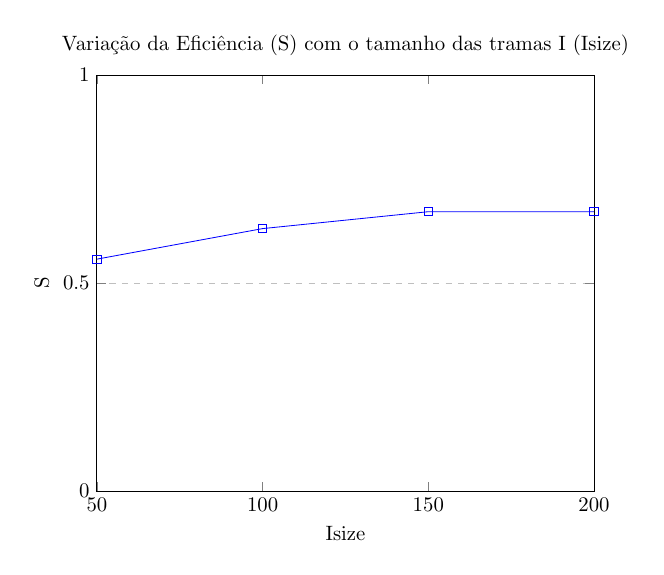
\begin{tikzpicture}[scale = 0.75]
    \begin{axis}[
        title={Variação da Eficiência (S) com o tamanho das tramas I (Isize)},
        xlabel={Isize},
        ylabel={S},
        xmin=50, xmax=200,
        ymin=0, ymax=1,
        xtick={0,50,100,150,200},
        ytick={0,0.5,1,1.5,2,2.5,3},
        legend pos=north west,
        ymajorgrids=true,
        grid style=dashed,
    ]
    
    \addplot[
        color=blue,
        mark=square,
        ]
        coordinates {
        (50,0.557589068)(100,0.631041149)(150,0.671663727)(200,0.671663727)
        };
        
    \end{axis}
    
\end{tikzpicture}
\end{center}

Por último conclui-se que o tamanho das tramas beneficia a eficiência mas apenas até um certo ponto, começando a estancar por volta dos 150 bytes.


    



\input{Conclusões}

\newpage
\section{Anexo 1}

\paragraph{Modules}

\begin{itemize}
    \item \textbf{application} - camada de aplicação
    \item \textbf{main} - interpretação dos argumentos de chamada
    \item \textbf{file} - interpretação e validação do nome de ficheiro dado
    \item \textbf{error} - simulação de erros e do tempo de propagação
    \item \textbf{state} machine - máquina de estados
    \item \textbf{data} link - protocolo de ligação de dados
    \item \textbf{macros} - constantes
\end{itemize}

\subsection{application.c}

\begin{lstlisting}[language=C, caption=application.c]
#include <stdio.h>
#include <unistd.h>
#include <fcntl.h>
#include <sys/stat.h>
#include <string.h>
#include <stdlib.h>
#include <stdint.h>
#include "file.h"
#include "data_link.h"
#include "application.h"

typedef struct {
    int file_descriptor;
    size_t transfer_file_size;
    ConnectionType status;
    char* transfer_file_name;
    char* transfer_file_dir;
    char* transfer_file_path;
} ApplicationLayer;

ApplicationLayer app_data;

int receiver(char* port_path);
int transmitter(char* port_path);

// RECEIVER AUX
size_t write_data_packet(uint8_t* data_packet, int fd, int* packet_no);
void parse_control_packet(uint8_t* packet);
int open_transfer_file();

// TRANSMITTER AUX
uint8_t* build_control_packet(size_t* control_packet_size, char* file_name);
size_t read_data_packet(int packetNo, uint8_t* data_packet, int fd, int bytes_read);
int read_file(char* file_path, uint8_t* buffer, size_t size);


void init_app(ConnectionType connection_type, char* file_path, char* serial_path) {
    app_data.transfer_file_name = calloc(FILE_NAME_SIZE, sizeof(char));
    app_data.transfer_file_dir = calloc(DIR_PATH_SIZE, sizeof(char));
    app_data.status = connection_type;
    
    path_parser(file_path, app_data.transfer_file_dir, app_data.transfer_file_name);

    if (connection_type == TRANSMITTER) {
        app_data.transfer_file_path = file_path;
        transmitter(serial_path);
    }
    if (connection_type == RECEIVER) {
        app_data.transfer_file_path = calloc(DIR_PATH_SIZE + FILE_NAME_SIZE, sizeof(char));
        receiver(serial_path);
        free(app_data.transfer_file_path);
    }

    free(app_data.transfer_file_dir);
    free(app_data.transfer_file_name);
}

void parse_control_packet(uint8_t* packet) {
    int i = 1;
    if (packet[i++] == 0x00) { // Filesize
        size_t file_size = 0;
        int n_bytes = (int) packet[i++];
        n_bytes--;
        while(n_bytes >= 0) {
            file_size += (size_t) packet[i++] << (n_bytes * 8);
            n_bytes--;
        }
        app_data.transfer_file_size = file_size;
    } else {
        fprintf(stderr, "Error in application - parse_control_packet: unexpected structure of the control_packet\n");
        exit(1);
    }
    if (packet[i++] == 0x01) { // Filename
        int n_bytes = (int) packet[i++];
        if (strlen(app_data.transfer_file_name) == 0) {
            strncpy(app_data.transfer_file_name, (char*) packet + i, n_bytes);
        }
        strncpy(app_data.transfer_file_path, app_data.transfer_file_dir, DIR_PATH_SIZE);
        strcat(app_data.transfer_file_path, app_data.transfer_file_name);
    } else {
        fprintf(stderr, "Error in application - parse_control_packet: unexpected structure of the control_packet\n");
        exit(1);
    }
}

size_t write_data_packet(uint8_t* data_packet, int fd, int* packet_no) {

    size_t packet_size = (size_t) (data_packet[2] << 8) + data_packet[3];
    if (*packet_no == (int) data_packet[1]) {
        (*packet_no)++;
    } else {
        fprintf(stderr, "Packet sequence number incorrect! Missed a packet\n");
        (*packet_no) = (int) data_packet[1] + 1;
    }

    if ((write(fd, data_packet + 4, packet_size * sizeof(uint8_t))) != packet_size) {
        perror("Error in application - write_data_packet");
        exit(1);
    }
    return packet_size;
}

int receiver(char* port_path) {

    int newFileDescriptor, packet_no = 0;
    size_t bytes_received = 0;
    bool fileOpen = false;
    uint8_t *data_packet;
    data_packet = calloc(MAX_PACKET_SIZE, sizeof(uint8_t));

    // OPEN
    if((app_data.file_descriptor = llopen(port_path, RECEIVER)) == -1) exit(1);

    printf("Receiver - connection established\n");
    
    while (true) {
        // READ
        if (llread(app_data.file_descriptor, data_packet, MAX_PACKET_SIZE) == -1) exit(1);
        if (data_packet[0] == 0x01) {
            bytes_received += write_data_packet(data_packet, newFileDescriptor, &packet_no);
            printf("Receiver - packet %d received\n", (int) data_packet[1]);
        } else if (data_packet[0] == 0x02) {
            parse_control_packet(data_packet);
            if (file_exists(app_data.transfer_file_dir, app_data.transfer_file_name)) {
                fprintf(stderr, "Error in application - receiver: file already exists\n");
                exit(1);
            }
            newFileDescriptor = open_transfer_file();
            fileOpen = true;

        } else if (data_packet[0] == 0x03) {
            // CLOSE
            if ((llclose(app_data.file_descriptor)) != 0) exit(1);
            printf("Receiver - connection cut\n");
            break;
        } else {
            fprintf(stderr, "Error in application - receiver: C byte value invalid\n");
            exit(1);
        }
    }

    if (bytes_received != app_data.transfer_file_size) {
        fprintf(stderr, "File size does not correspond to the expected\n");
    }

    if (fileOpen) {
        if ((close(newFileDescriptor) == -1)) {
            perror("Error in application - receiver");
            exit(1);
        }
    }
    free(data_packet);
    
    return 0;
}

size_t read_data_packet(int packetNo, uint8_t* data_packet, int fd, int bytes_read) {
    size_t bytes_to_write = (MAX_PACKET_SIZE > (app_data.transfer_file_size - bytes_read + 4)) ? (app_data.transfer_file_size - bytes_read) : MAX_PACKET_SIZE - 4; // In case of the file being in its end
    data_packet[0] = 0x01;
    data_packet[1] = (uint8_t) packetNo;
    data_packet[2] = (uint8_t) (bytes_to_write & 0xFF00) >> 8; // Amount of data
    data_packet[3] = (uint8_t) bytes_to_write & 0x00FF;
    if ((read(fd, data_packet + 4, bytes_to_write * sizeof(uint8_t))) != bytes_to_write) {
        perror("Error in application - read_data_packet");
        exit(1);
    }
    return bytes_to_write + 4;
}

uint8_t* build_control_packet(size_t* control_packet_size, char* file_name) {
    size_t file_name_size = strlen(file_name) + 1; //To actually copy \0

    if (file_name_size > MAX_PACKET_SIZE - 13) {
        fprintf(stderr, "Error in application - build_control_packet: filename too big\n");
        exit(1);
    }

    *control_packet_size = file_name_size + 13;
    uint8_t* buffer = calloc((*control_packet_size), sizeof(uint8_t));

    buffer[0] = 0x02; // C
    buffer[1] = 0; // T
    buffer[2] = (uint8_t) sizeof(app_data.transfer_file_size); // L
    buffer[3] = (app_data.transfer_file_size & 0xFF00000000000000) >> 56; // filesize
    buffer[4] = (app_data.transfer_file_size & 0x00FF000000000000) >> 48;
    buffer[5] = (app_data.transfer_file_size & 0x0000FF0000000000) >> 40;
    buffer[6] = (app_data.transfer_file_size & 0x000000FF00000000) >> 32;
    buffer[7] = (app_data.transfer_file_size & 0x00000000FF000000) >> 24;
    buffer[8] = (app_data.transfer_file_size & 0x0000000000FF0000) >> 16;
    buffer[9] = (app_data.transfer_file_size & 0x000000000000FF00) >> 8;
    buffer[10] = app_data.transfer_file_size & 0x00000000000000FF;
    buffer[11] = 1; // T
    buffer[12] = (uint8_t) (sizeof(char) * file_name_size); // L
    memcpy((char*) buffer + 13, file_name, file_name_size); // filename
    return buffer;
}

int transmitter(char* port_path) {
    uint8_t *control_packet, *data_packet;
    struct stat s;
    size_t control_packet_size, bytes_read = 0, bytes_written;
    int packet_no = 0, oldFileDescriptor;

    if (stat(app_data.transfer_file_path, &s) == -1) {
        perror("Error in application - transmitter - stat");
        exit(1);
    }
    app_data.transfer_file_size = s.st_size;
    data_packet = calloc(MAX_PACKET_SIZE, sizeof(uint8_t));

    oldFileDescriptor = open_transfer_file();

    // OPEN
    if( (app_data.file_descriptor = llopen(port_path, TRANSMITTER)) == -1) exit(1);
    control_packet = build_control_packet(&control_packet_size, app_data.transfer_file_name);

    printf("Transmitter - connection established\n");

    // START
    if ((llwrite(app_data.file_descriptor, control_packet, control_packet_size)) == -1) exit(1); 

    printf("Transmitter - transmition begun\n");

    // WRITING
    while (bytes_read < app_data.transfer_file_size) {
        packet_no++;
        bytes_written = read_data_packet(packet_no, data_packet, oldFileDescriptor, bytes_read);
        bytes_read += bytes_written - 4;
        if ((llwrite(app_data.file_descriptor, data_packet, bytes_written)) == -1) exit(1);
        printf("Transmitter - packet %d sent\n", packet_no);
    }

    // FINISH
    control_packet[0] = 0x03;
    if ((llwrite(app_data.file_descriptor, control_packet, control_packet_size)) == -1) {
        fprintf(stderr, "Error in application - transmitter - fatal error when writting control packet\n");
        exit(1);
    } 

    printf("Transmitter - transmition ended\n");

    // CLOSE
    if ((llclose(app_data.file_descriptor)) != 0) exit(1);

    printf("Transmitter - connection cut\n");

    if ((close(oldFileDescriptor) == -1)) {
        perror("Error in application - transmitter");
        exit(1);
    }

    free(data_packet);
    free(control_packet);  

    return 0;
}

int open_transfer_file() {
    int fd;

    switch (app_data.status) {
        case TRANSMITTER: {
            if ((fd = open(app_data.transfer_file_path, O_RDONLY)) == -1) {
                perror("Error in application - transmitter - open_transfer_file");
                exit(1);
            }
            break;
        }
        case RECEIVER: {
            if ((fd = creat(app_data.transfer_file_path, S_IRUSR | S_IWUSR | S_IRGRP | S_IROTH)) == -1) {
                perror("Error in application - receiver - open_transfer_file");
                exit(1);
            }
            break;
        }

        default: {
            fprintf(stderr, "Error in application - open_transfer_file: wrong type of connection\n");
            exit(1);
        }
    }
    return fd;
}
\end{lstlisting}

\subsection{application.h}

\begin{lstlisting}[language=C, caption=application.h]
#pragma once

#include "macros.h"

void init_app(ConnectionType connection_type, char* file_path, char* serial_path);

\end{lstlisting}

\subsection{main.c}

\begin{lstlisting}[language=C, caption=main.c]
#include <stdio.h>
#include <stdlib.h>
#include <stdbool.h>
#include <getopt.h>
#include <time.h>
#include "error.h"
#include "state_machine.h"
#include "application.h"

void print_cmd_args() {
    printf("Usage: \n");
    printf("    rcompy -r/-t --file <argument> --serial_port <argument> [--fer <argument> --t_prop <argument> --help]\n");
    printf("Options: \n");
    printf("    -r               Receiver mode\n");
    printf("    -t               Transmitter mode\n");
    printf("    -f --file        Choose destination if receiver or source if transmitter\n");
    printf("    -s --serial_port Choose serial port path\n");
    printf("    -z --header_error_ratio        Choose error generation probability in information packets\n");
    printf("    -x --data_error_ratio         Choose error generation probability in information packets\n");
    printf("    -p --t_prop      Choose propagation delay in milliseconds\n");
    printf("    -h --help        Show this help message\n");
}

// Just parsing
int main(int argc, char** argv) {
    
    srandom(time(NULL));
    struct option options[] = {
        {"file", required_argument, 0, 'f'},
        {"serial_port", required_argument, 0, 's'},
        {"header_error_ratio", required_argument, 0, 'z'},
        {"data_error_ratio", required_argument, 0, 'x'},
        {"t_prop", required_argument, 0, 'p'},
        {"help", required_argument, 0, 'h'},
        {0, 0, 0, 0}
    };

    bool is_trans, is_rec, had_file_path, had_serial_path, had_header_error, had_data_error, had_tprop;
    is_trans = is_rec = had_file_path = had_serial_path = had_header_error = had_data_error = had_tprop = false;

    char* file_path;
    char* serial_port_path;
    int t_prop = 0;
    double header_error = 0;
    double data_error = 0;

    int c = 0;
    int opt_index = 0;
    while((c = getopt_long(argc, argv, "htrf:p:x:z:s:", options, &opt_index)) != -1) {
        switch (c) {
            case 't': {
                is_trans = true;
                if (is_rec) {
                    print_cmd_args();
                    return 1;
                }
                break;
            }
            case 'r': {
                is_rec = true;
                if (is_trans) {
                    print_cmd_args();
                    return 1;
                }
                break;
            }
            case 'f': {
                if (had_file_path) {
                    print_cmd_args();
                    return 1;
                }
                had_file_path = true;
                file_path = optarg;
                break;
            }
            case 's': {
                if (had_serial_path) {
                    print_cmd_args();
                    return 1;
                }
                had_serial_path = true;
                serial_port_path = optarg;
                break;
            }
            case 'p': {
                if (had_tprop) {
                    print_cmd_args();
                    return 1;
                }
                had_tprop = true;
                t_prop = atoi(optarg);
                break;
            }
            case 'z': {
                if (had_header_error) {
                    print_cmd_args();
                    return 1;
                }
                had_header_error = true;
                header_error = strtod(optarg, NULL);
                break;
            }
            case 'x': {
                if (had_data_error) {
                    print_cmd_args();
                    return 1;
                }
                had_data_error = true;
                data_error = strtod(optarg, NULL);
                break;
            }
            case 'h': {
                print_cmd_args();
                return 1;
            }
            default: {
                print_cmd_args();
                return 1;
            }
        }
    }
    if (!had_file_path || !had_serial_path || (!is_rec && !is_trans)) {
        print_cmd_args();
        return 1;
    }

    set_error_rates(header_error, data_error);
    set_prop_time(t_prop);
    init_app(is_rec ? RECEIVER : TRANSMITTER, file_path, serial_port_path);

    return 0;
}
\end{lstlisting}

\subsection{data \textunderscore link.c}

\begin{lstlisting}[language=C, caption=data_link.c]
#include <unistd.h>
#include <stdio.h>
#include <string.h>
#include <fcntl.h>
#include <strings.h>
#include <termios.h>
#include <stdbool.h>
#include "data_link.h"
#include "alarm.h"
#include "state_machine.h"
#include "macros.h"


static struct termios old_terminal;
static struct LinkLayerData link_layer_data;
static uint8_t* aux_buffer;
static bool alarm_called = false;

int setup_terminal(int fd);
int restore_terminal(int fd);

int assemble_supervision_frame(FrameType frame_type, ConnectionType connection_type, uint8_t* frame_buffer);
uint32_t assemble_information_frame(uint8_t* packet_data, size_t packet_size, uint8_t* frame, uint8_t frame_number);
int write_buffer(int fd, uint8_t* buffer, size_t length, FrameType expected_response);
bool validBCC2(uint8_t bcc2, uint8_t* buffer, size_t buffer_size);
uint8_t compute_bcc2(uint8_t* buffer, size_t buffer_size);

int establish_transmitter_connection(int fd);
int wait_transmitter_connection(int fd);
int disconnect_transmitter(int fd);
int disconnect_receiver(int fd);

void dl_alarm_callback() {
    alarm_called = true;
}

int llopen(char* port, ConnectionType role) {

    int fd = 0;
    alarm_called = false;

    // Configure port
    snprintf(link_layer_data.port, sizeof(char)*MAX_PORT_SIZE, "%s", port);
    link_layer_data.role = role;
    link_layer_data.baud_rate = BAUDRATE;
    link_layer_data.num_transmissions = NUM_TX;
    link_layer_data.timeout = TIMEOUT;

    if ((link_layer_data.frame = calloc(MAX_FRAME_SIZE, sizeof(uint8_t))) == NULL) {
        return -1;
    }
    if ((aux_buffer = calloc(MAX_FRAME_SIZE + 1, sizeof(uint8_t))) == NULL) {
        return -1;
    }

    fd = open(link_layer_data.port, O_RDWR | O_NOCTTY );
    if (fd < 0) {
        perror("Error in data_link - llopen - opening port");
        return -1;
    } 

    if (setup_terminal(fd) == -1) {
        perror("Error in data_link - llopen");
        return -1;
    }

    if (setup_alarm_handler() == -1) {
        fprintf(stderr, "Error in data_link - llopen: setting up alarm handler\n");
        return -1;
    }

    if (subscribe_alarm(dl_alarm_callback) == -1) { // Subscribing a specific function to be called in alarm
        fprintf(stderr, "Error in data_link - llopen: subscribing alarm event\n");
        return -1;
    }

    switch(role) {
        case TRANSMITTER: {
            if ((establish_transmitter_connection(fd)) == -1) return -1;
            break;
        }
        case RECEIVER: {
            if ((wait_transmitter_connection(fd)) == -1) return -1;
            break;
        }
        default: {
            fprintf(stderr, "Error in data_link - llopen: tried to open a connection with invalid role\n");
            return -1;
        }
    }

    return fd;   
}

int llclose(int fd) {
    if (link_layer_data.role == TRANSMITTER) {
        disconnect_transmitter(fd);
    } else if (link_layer_data.role == RECEIVER) {
        disconnect_receiver(fd);
    }
    if (restore_terminal(fd) == -1) {
        perror("Error in data_link - llclose");
        return -1;
    }
    if (restore_alarm_handler() == -1) {
        fprintf(stderr, "Error in data_link - llclose: restoring alarm handlers\n");
        return -1;
    }
    free(aux_buffer);
    free(link_layer_data.frame);
    return close(fd);
}

int llwrite(int fd, uint8_t* packet, size_t packet_length) {
    static uint8_t package_to_send = 0;
    uint8_t frame_length;
    FrameType expected_response;

    // Numero de sequência
    if (package_to_send == 0) {
        expected_response = RR_1;
        frame_length = assemble_information_frame(packet, packet_length, link_layer_data.frame, 0);
    } else {
        expected_response = RR_0;
        frame_length = assemble_information_frame(packet, packet_length, link_layer_data.frame, 1);
    }

    // Writing
    int res = write_buffer(fd, link_layer_data.frame, frame_length, expected_response);
    if ( res == -2) {
        fprintf(stderr, "Error in data_link - llwrite: no. tries exceeded\n");
        return -1;
    } else if ( res == -1) {
        perror("Error in data_link - llwrite");
        return -1;
    } else if ( res != frame_length) {
        fprintf(stderr, "Error in data_link - llwrite: no. bytes written not matching expected\n");
        return -1;
    }
    package_to_send = package_to_send ? 0 : 1;
    return res;
}

/*
    This function reads into a buffer a packet that was read from the serial port
    fd -> Serial port file descriptor
    buffer -> Buffer that will receive the packet
    max_buffer_size -> Max size of buffer variable, used to check if a packet can fit into the provided buffer
*/
int llread(int fd, uint8_t* buffer, size_t max_buffer_size) {
    if (max_buffer_size < MAX_PACKET_SIZE) {

        fprintf(stderr, "Error in data_link - llread: provided buffer does not meet size requirements\n");
        return -1;
    }

    size_t frame_size;
    static uint8_t expected_package;
    uint8_t response_frame[SUPV_FRAME_SIZE];
    StateMachineResult new_frame;
    bool valid_frame = false;

    while(!valid_frame) {

        new_frame = read_frame(fd, link_layer_data.frame, MAX_FRAME_SIZE);
        frame_size = destuff(link_layer_data.frame, new_frame.packet_size, aux_buffer, MAX_PACKET_SIZE + 1);

        if (frame_size == 0) {
            fprintf(stderr, "Error in data_link - llread: destuffing packet unsuccessfull\n");
            return -1;
        }
        uint8_t bcc2 = aux_buffer[--frame_size];

        // Error
        if (new_frame.frame_type != expected_package || !validBCC2(bcc2, aux_buffer, frame_size)) {
            if (assemble_supervision_frame(expected_package ? REJ_1 : REJ_0, RECEIVER, response_frame) == -1) return -1;
        } else {
            memcpy(buffer, aux_buffer, frame_size);
            if (assemble_supervision_frame(expected_package ? RR_0 : RR_1, RECEIVER, response_frame) == -1) return -1;
            valid_frame = true;
        }
        if (write(fd, response_frame, SUPV_FRAME_SIZE) != 5) {
            fprintf(stderr, "Error in data_link - llread: did not write response frame correctly");
            return -1;
        }
    }

    expected_package = expected_package ? 0 : 1;
    return frame_size;
}

int setup_terminal(int fd) {
    struct termios new_terminal;

    if ( tcgetattr(fd, &old_terminal) == -1) {
      return -1;
    }

    bzero(&new_terminal, sizeof(new_terminal));
    new_terminal.c_cflag = link_layer_data.baud_rate | CS8 | CLOCAL | CREAD;
    new_terminal.c_iflag = IGNPAR;
    new_terminal.c_oflag = 0;
    new_terminal.c_lflag = 0;

    new_terminal.c_cc[VTIME] = VTIME_VALUE;
    new_terminal.c_cc[VMIN] = VMIN_VALUE;

    tcflush(fd, TCIOFLUSH);

    if ( tcsetattr(fd,TCSANOW,&new_terminal) == -1) {
      return -1;
    }
     
    return 0;
}

int restore_terminal(int fd) {
    if (tcsetattr(fd,TCSANOW,&old_terminal) == -1) {
      return -1;
    }
    return 0;
}

int assemble_supervision_frame(FrameType frame_type, ConnectionType connection_type, uint8_t* frame_buffer) {
    frame_buffer[0] = FLAG;
    switch (connection_type) {
        case TRANSMITTER: {
            frame_buffer[1] = 0x03;
            if (frame_type == UA) {
                frame_buffer[1] = 0x01;
            } 
            if (frame_type == SET || frame_type == DISC || frame_type == UA) {
                frame_buffer[2] = frame_type;
            } else {
                fprintf(stderr, "Error: Data_link - assemble_supervision_frame - invalyd frame_type: %x\n", frame_type);
                return -1; //Invalid frame_type for this function
            }
            break;
        }
        case RECEIVER: {
            frame_buffer[1] = 0x03;
            if (frame_type == DISC) {
                frame_buffer[1] = 0x01;
            } 
            if (frame_type == UA || frame_type == DISC || frame_type == RR_0 || frame_type == RR_1 || frame_type == REJ_0 || frame_type == REJ_1) {
                frame_buffer[2] = frame_type;
            } else {
                fprintf(stderr, "Error: Data_link - assemble_frame - invalyd frame_type\n");
                return -1; //Invalid frame_type for this function
            }
            break;
        }
    }
    frame_buffer[3] = frame_buffer[1] ^ frame_buffer[2];
    frame_buffer[4] = FLAG;
    return 0;
}

uint32_t assemble_information_frame(uint8_t* packet_data, size_t packet_size, uint8_t* frame, uint8_t frame_number) {
    size_t frame_size = 4;
    frame[0] = FLAG;
    frame[1] = 0x03;
    frame[2] = frame_number;
    frame[3] = frame[1] ^ frame[2];
    frame_size = stuff(packet_data, packet_size, frame, frame_size);
    uint8_t bcc2[2];
    bcc2[0] = compute_bcc2(packet_data, packet_size);
    frame_size = stuff(bcc2, 1, frame, frame_size);
    frame[frame_size++] = FLAG;
    return frame_size;
}

uint32_t stuff(uint8_t* packet, size_t length, uint8_t* frame, size_t occupied_bytes) {
    size_t stuffed_length = occupied_bytes;

    int new_buffer_i = occupied_bytes;

    for (int i = 0; i < length; i++) {
        uint8_t byte = packet[i];
        if (byte == FLAG || byte == ESC_HEX) {
            frame[new_buffer_i++] = ESC_HEX;
            frame[new_buffer_i++] =  byte ^ STUFF_XOR_HEX;
            stuffed_length++;
        } else {
            frame[new_buffer_i++] = byte;
        }
        stuffed_length++;
    }
    return stuffed_length;
}

uint32_t destuff(uint8_t* stuffed_packet, size_t stuffed_length, uint8_t* unstuffed_packet, size_t max_unstuffed_packet_size) {
    size_t unstuffed_length = stuffed_length;

    int64_t new_buffer_i = 0;

    for (int i = 0; i < stuffed_length; i++) {
        uint8_t byte = stuffed_packet[i];
        if (new_buffer_i >= max_unstuffed_packet_size) {
            fprintf(stderr, "Error in data_link - destuffing: unstuffed packet is bigger than the destiny buffer! Tried to access %ld on a %ld bytes buffer\n", new_buffer_i, max_unstuffed_packet_size);
            return 0;
        }
        if (byte == ESC_HEX && i < stuffed_length - 1) {
            if (stuffed_packet[i + 1] == (FLAG ^ STUFF_XOR_HEX)) {
                unstuffed_packet[new_buffer_i++] = FLAG;
            } else if (stuffed_packet[i + 1] == (ESC_HEX ^ STUFF_XOR_HEX)) {
                unstuffed_packet[new_buffer_i++] = ESC_HEX;
            }
            unstuffed_length--;
            i++;
        } else {
            unstuffed_packet[new_buffer_i++] = byte;
        }
    }
    return unstuffed_length;
}

int establish_transmitter_connection(int fd) {
    uint8_t supervision_buffer[SUPV_FRAME_SIZE];
    
    if ((assemble_supervision_frame(SET, TRANSMITTER, supervision_buffer)) != 0) {
        return -1;
    }
    int res = write_buffer(fd, supervision_buffer, SUPV_FRAME_SIZE, UA);
    if (res == -2) {
        fprintf(stderr, "Error in data_link - establish_transmitter_connection: no. tries exceeded\n");
        return -1;
    } else if ( res == -1) {
        perror("Error in data_link - disconnect_receiver");
        return -1;
    } else if (res != 5) {
        fprintf(stderr, "Error in data_link - establish_transmitter_connection: no. bytes written not matching expected\n");
        return -1;
    }
    return 0;
}

int wait_transmitter_connection(int fd) {
    StateMachineResult res = read_frame(fd, link_layer_data.frame, MAX_FRAME_SIZE);
    if (res.frame_type == SET) {
        uint8_t supervision_buffer[SUPV_FRAME_SIZE];
        assemble_supervision_frame(UA, RECEIVER, supervision_buffer);
        if (write(fd, supervision_buffer, SUPV_FRAME_SIZE) != 5) {
            fprintf(stderr, "Error in data_link - wait_transmiiter_connection: could no write ACK to transmitter\n");
            return -1;
        }
        return 0;
    } else {
        fprintf(stderr, "Error in data_link - wait_transmiiter_connection: received wrong type of frame\n");
        return -1;
    }
}

int disconnect_transmitter(int fd) {
    uint8_t supervision_buffer[SUPV_FRAME_SIZE];
    assemble_supervision_frame(DISC, TRANSMITTER, supervision_buffer);
    int res = write_buffer(fd, supervision_buffer, SUPV_FRAME_SIZE, DISC); 
    if ( res == -2) {
        fprintf(stderr, "Error in data_link - disconnect_transmitter: no. tries exceeded\n");
        return -1;
    } else if ( res == -1) {
        perror("Error in data_link - disconnect_receiver");
        return -1;
    } else if ( res != 5) {
        fprintf(stderr, "Error in data_link - disconnect_transmitter: no. bytes written not matching expected\n");
        return -1;
    }
    assemble_supervision_frame(UA, TRANSMITTER, supervision_buffer);
    if (write(fd, supervision_buffer, SUPV_FRAME_SIZE) != 5) {
        return -1;
    }
    return 0;
}

int disconnect_receiver(int fd) {

    StateMachineResult res = read_frame(fd, link_layer_data.frame, MAX_FRAME_SIZE);
    if (res.frame_type == DISC) {
        uint8_t supervision_buffer[SUPV_FRAME_SIZE];
        assemble_supervision_frame(DISC, TRANSMITTER, supervision_buffer);
        int res = write_buffer(fd, supervision_buffer, SUPV_FRAME_SIZE, UA); 
        if ( res == -2) {
            fprintf(stderr, "Error in data_link - disconnect_receiver: no. tries exceeded\n");
            return -1;
        } else if ( res == -1) {
            perror("Error in data_link - disconnect_receiver");
            return -1;
        } else if ( res != 5) {
            fprintf(stderr, "Error in data_link - disconnect_receiver: no. bytes written not matching expected\n");
            return -1;
        }
        return 0;
    } else {
        fprintf(stderr, "Error in data_link - disconnect_receiver: unexpected frame type\n");
        return -1;
    }
}

/* Writes a buffer to the serial port and awaits a certain response
    fd -> Serial port file desciptor
    buffer -> buffer to write
    length -> length of the buffer to be written
    expected_response -> expected response sent by the other end of the serial port
*/
int write_buffer(int fd, uint8_t* buffer, size_t length, FrameType expected_response) {
    StateMachineResult res_frame = {};
    int tries = NUM_TX;
    int res = 0;
    while (tries > 0) {
        if((res = write(fd, buffer, length * sizeof(uint8_t))) == -1) return -1; // Writes buffer to serial port
        alarm(3);
        res_frame = read_frame(fd, link_layer_data.frame, MAX_FRAME_SIZE); // Reads response
        if (alarm_called) { // Timeout
            tries--;
            alarm_called = !alarm_called;
            fprintf(stderr, "Alarm called, response timed out, %d tries left\n", tries);
        } else {
            alarm(0);
            if (res_frame.frame_type == expected_response) {
                //Only break if frame received and data was correct
                break;
            }
        }
    }
    if (tries <= 0) { // Timeout limit 
        return -2;
    } else {
        return res;
    }
}

bool validBCC2(uint8_t bcc2, uint8_t* buffer, size_t buffer_size) {
    uint8_t side_bcc2 = compute_bcc2(buffer, buffer_size);
    return ((side_bcc2 ^ bcc2) == 0);
}

uint8_t compute_bcc2(uint8_t* buffer, size_t buffer_size) {
    uint8_t bcc2 = buffer[0];
    for (int i = 1; i < buffer_size; i++) {
        bcc2 ^= buffer[i];
    }
    return bcc2;
}

\end{lstlisting}

\subsection{data \textunderscore link.h}

\begin{lstlisting}[language=C, caption=data_link.h]
#pragma once

#include <stdlib.h>
#include <stdint.h>
#include <stdbool.h>
#include "macros.h"
#include "state_machine.h"

#define MAX_FRAME_SIZE ((MAX_PACKET_SIZE * 2) + 7)

struct LinkLayerData {
    ConnectionType role;
    char port[MAX_PORT_SIZE];
    unsigned int baud_rate;
    unsigned int sequence_number;
    unsigned int timeout;
    unsigned int num_transmissions;
    uint8_t* frame;
} LinkLayerData;

uint32_t stuff(uint8_t* packet, size_t length, uint8_t* frame, size_t occupied_bytes);
uint32_t destuff(uint8_t* stuffed_packet, size_t stuffed_length, uint8_t* unstuffed_packet, size_t max_unstuffed_packet_size);

int llopen(char* port, ConnectionType role);
int llwrite(int fd, uint8_t* buffer, size_t length);
int llread(int fd, uint8_t* buffer, size_t max_buffer_size);
int llclose(int fd);

\end{lstlisting}

\subsection{alarm.c}

\begin{lstlisting}[language=C, caption=alarm.c]
#include <stdio.h>
#include <stdlib.h>
#include <signal.h>
#include <stdbool.h>
#include "alarm.h"

static struct sigaction old_action;
static AlarmListener* alarm_listeners = NULL; 
static size_t number_of_listeners = 0;

// Alarm handler
void alarm_callback(int signo) {
    // Calls 'subhandlers' that were subscribed (behaviour like observer pattern in OP)
    for (int i = 0; i < number_of_listeners; i++) {
        alarm_listeners[i]();
    }
}

int setup_alarm_handler() {
    struct sigaction new_action;
    sigset_t smask;
    if (sigemptyset(&smask)==-1) {
        return -1;
    }

    new_action.sa_mask = smask;
    new_action.sa_handler = alarm_callback;
    new_action.sa_flags = 0;

    if (sigaction(SIGALRM, &new_action, &old_action) == -1) {
        perror("Error in alarm - setup_alarm_handler");
        return -1;
    }
    return 0;
}

// Add a new subhandler/listener to the functions to be called when the alarm 'rings'
int subscribe_alarm(AlarmListener alarm_listener) {
    number_of_listeners++;
    if (alarm_listeners == NULL) {
        if ((alarm_listeners = (AlarmListener*) malloc(sizeof(AlarmListener))) == NULL) {
            perror("Error in alarm - subscribe_alarm");
            return -1;
        }
        alarm_listeners[0] = alarm_listener;
    } else {
        AlarmListener* new_alarm_listeners;
        if ((new_alarm_listeners = realloc(alarm_listeners, sizeof(AlarmListener) * number_of_listeners)) == NULL) {
            perror("Error in alarm - subscribe_alarm");
            return -1;
        }
        alarm_listeners = new_alarm_listeners;
        alarm_listeners[number_of_listeners - 1] = alarm_listener;
    }
    return 0;
}

int restore_alarm_handler() {
    free(alarm_listeners);
    number_of_listeners = 0;
    if (sigaction(SIGALRM, &old_action, NULL) == -1) {
        return -1;
    }
    return 0;
}

\end{lstlisting}

\subsection{alarm.h}

\begin{lstlisting}[language=C, caption=alarm.h]
#pragma once

typedef void (*AlarmListener)(); 

int setup_alarm_handler();
int subscribe_alarm(AlarmListener alarm_listener);
int restore_alarm_handler();

\end{lstlisting}

\subsection{error.c}

\begin{lstlisting}[language=C, caption=error.c]
#include <unistd.h>
#include <stdio.h>
#include <stdlib.h>
#include "error.h"
#include "macros.h"


static double header_error_rate = 0;
static double data_error_rate = 0;
static int prop_time = 0;


bool should_corrupt(double error_rate);
uint8_t gen_corrupted_byte();




bool should_corrupt(double error_rate) {
    double prob = (double) random()/ (double) RAND_MAX;
    return (prob <= error_rate);
}

bool should_corrupt_data() {
    return should_corrupt(data_error_rate);
}

bool should_corrupt_header() {
    return should_corrupt(header_error_rate);
}

void corrupt_header(uint8_t* a, uint8_t* c, uint8_t* bcc1) {
    printf("Generated header error\n");
    uint64_t corrupted_byte = random() % 3;
    switch (corrupted_byte) {
        case 0:
            *a = gen_corrupted_byte();
            break;
        case 1:
            *c = gen_corrupted_byte();
            break;
        case 2:
            *bcc1 = gen_corrupted_byte();
            break;
        default:
            fprintf(stderr, "Error in error.c - corrupt_header: unexpected corrupted_byte\n");
            break;
    }
}

void corrupt_data_buffer(uint8_t* data_buffer, size_t buffer_size) {
    printf("Generated data error\n");
    size_t corrupted_byte_idx = random() % buffer_size;
    data_buffer[corrupted_byte_idx] = gen_corrupted_byte();
}

uint8_t gen_corrupted_byte() {
    return ((uint8_t) random());
}

void set_error_rates(double h_error, double d_error) {
    header_error_rate = h_error;
    data_error_rate = d_error;
}

void set_prop_time(int t_prop) {
    prop_time = t_prop;
}

void delay() {
    usleep(1000*prop_time);
}

\end{lstlisting}

\subsection{error.h}

\begin{lstlisting}[language=C, caption=error.h]
#pragma once

#include <stdbool.h>
#include <stdint.h>


void delay();
void set_error_rates(double h_error, double d_error);
void set_prop_time(int t_prop);
bool should_corrupt_data();
bool should_corrupt_header();
void corrupt_header(uint8_t* a, uint8_t* c, uint8_t* bcc1);
void corrupt_data_buffer(uint8_t* data_buffer, size_t buffer_size);
\end{lstlisting}

\subsection{macros.h}

\begin{lstlisting}[language=C, caption=macros.h]
#pragma once

typedef enum { TRANSMITTER, RECEIVER } ConnectionType;

#define _POSIX_SOURCE 1 /* POSIX compliant source */
#define FLAG 0x7E
#define BAUDRATE B38400
#define NUM_TX 3 //Number of tries
#define VMIN_VALUE 5
#define VTIME_VALUE 0
#define TIMEOUT 2 //Timeout in seconds
#define FALSE 0
#define TRUE 1
#define MAX_PACKET_SIZE 150
#define MAX_PORT_SIZE 20
#define SUPV_FRAME_SIZE 5
#define INF_DATA_LAYER_SIZE 6
#define STUFF_XOR_HEX 0x20
#define ESC_HEX 0x7d

\end{lstlisting}

\subsection{state \textunderscore machine.c}

\begin{lstlisting}[language=C, caption=state_machine.c]
#include <stdbool.h>
#include <stdio.h>
#include <unistd.h>
#include <stdlib.h>
#include "error.h"
#include "macros.h"
#include "alarm.h"
#include "state_machine.h"

enum StateType_ {START, FLAG_RCV, A_RCV, C_RCV, BCC_OK, DATA, STOP};
typedef enum StateType_ StateType;

/*
    Functions declared here because they are private
*/
bool isA(uint8_t a);
bool isC(uint8_t c);

// State machine to read the serial port and check the input validity
StateMachineResult read_frame(int fd, uint8_t* frame, size_t frame_size) {
    StateMachineResult state_machine_res  = {
        .frame_type = ERROR,
        .packet_size = 0,
    };
    uint8_t byte_rcvd, a, c;
    StateType state = START;
    a = byte_rcvd = c = 0;

    while (state != STOP) {
        if(read(fd, &byte_rcvd, sizeof(uint8_t)) == -1) {
            return state_machine_res;
        }
        switch (state) {
            case START: {
                if (byte_rcvd == FLAG) {
                    state = FLAG_RCV;
                }
                break;
            }
            case FLAG_RCV: {
                if (isA(byte_rcvd)) {
                    a = byte_rcvd;
                    state = A_RCV;
                } else if (byte_rcvd != FLAG) {
                    state = START;
                }
                break;
            }
            case A_RCV: {
                if (isC(byte_rcvd)) {
                    c = byte_rcvd;
                    state = C_RCV;
                } else if (byte_rcvd == FLAG) {
                    state = FLAG_RCV;
                } else {
                    state = START;
                }
                break;
            }
            case C_RCV: {
                if ((c == I_0 || c == I_1) && should_corrupt_header()) {
                    corrupt_header(&a, &c, &byte_rcvd);
                }
                if ((a ^ c ^ byte_rcvd) == 0) {
                    state = BCC_OK;
                } else if (byte_rcvd == FLAG) {
                    state = FLAG_RCV;
                } else {
                    state = START;
                }
                break;
            }
            case BCC_OK: {
                if (byte_rcvd == FLAG) {
                    state = STOP;
                } else {
                    state_machine_res.packet_size++;
                    frame[0] = byte_rcvd;
                    state = DATA;
                }
                break;
            }
            case DATA: {
                if (byte_rcvd == FLAG) {
                    state = STOP;
                } else {
                    state_machine_res.packet_size++;
                    if (state_machine_res.packet_size == frame_size) {
                        fprintf(stderr, "Error in data_link - state_machine: receiving more bytes than the max frame size\n");
                        return state_machine_res;
                    } 
                    frame[state_machine_res.packet_size - 1] = byte_rcvd;
                }
                break;
            }
            case STOP:
                break;
        }
    }
    state_machine_res.frame_type = c;

    // Random errors
    if ((state_machine_res.frame_type == I_0 || state_machine_res.frame_type == I_1) && should_corrupt_data()) {
        corrupt_data_buffer(frame, state_machine_res.packet_size);
    }

    delay(); // T_PROP

    return state_machine_res;
}

bool isA(uint8_t a) {
    return (a == 0x03) || (a == 0x01);
}

bool isC(uint8_t c) {
    c &= 0x0F; // Removes useless package data
    return (c == SET) || (c == DISC) || (c == UA) || (c == RR_0) || (c == REJ_0) || (c == I_0) || (c == I_1);
}





\end{lstlisting}

\subsection{state \textunderscore machine.h}

\begin{lstlisting}[language=C, caption=state_machine.h]
#pragma once

#include <stdlib.h>
#include <stdint.h>

typedef enum {SET=0x03, UA=0x07, I_0 = 0x00, I_1 = 0x01, RR_0=0x05, RR_1=0x85, DISC=0x0D, ERROR, REJ_0=0x01, REJ_1=0x81, NONE} FrameType;

typedef struct {
    FrameType frame_type;
    size_t packet_size;
} StateMachineResult;

StateMachineResult read_frame(int fd, uint8_t* frame, size_t frame_size); 
\end{lstlisting}

\subsection{file.c}

\begin{lstlisting}[language=C, caption=file.c]
#include <stdio.h>
#include <stdlib.h>
#include <stdint.h>
#include <string.h>
#include <errno.h>
#include <sys/stat.h>
#include <fcntl.h>
#include "file.h"

// Create Dir and Path for file
int path_parser(char* path, char* dir, char* file_name) {
    file_name[0] = '\0';
    dir[0] = '\0';

    char* last_dir_sep = strrchr(path, '/');
    char* cur_ptr = path;

    // Dir separation
    if (last_dir_sep == NULL) {
        strcpy(dir, "./");
        strcpy(file_name, path);
    } else {    
        char* cur_ptr = path;
        size_t dir_idx = 0;
        while (cur_ptr != last_dir_sep) {
            dir[dir_idx] = *cur_ptr;
            cur_ptr++;
            dir_idx++;
        }
        dir[dir_idx] = '/';
        dir[dir_idx + 1] = '\0';
        cur_ptr = ++last_dir_sep;
    }
    
    // Path separation
    size_t file_name_idx = 0;
    while (*cur_ptr != '\0') {
        file_name[file_name_idx] = *cur_ptr;
        cur_ptr++;
        file_name_idx++;
    }
    *cur_ptr = '\0';

    struct stat stat_buf;
    int status;
    if ((status = stat(dir, &stat_buf)) == -1) {
        perror("Error in path_parser");
        return -1;
    }
    if (S_ISDIR(stat_buf.st_mode)) {
        return 0;
    } else if (S_ISREG(stat_buf.st_mode)) {
        fprintf(stderr, "Error in path_parser - file already exists!\n");
        return -1;
    } else {
        fprintf(stderr, "Error in path_parser - nvalid file path\n");
        return -1;
    }
    
}

bool file_exists(char* dir, char* file_name) {
    char* file_path = calloc(DIR_PATH_SIZE + FILE_NAME_SIZE, sizeof(uint8_t));
    strncpy(file_path, dir, DIR_PATH_SIZE);
    strcat(file_path, file_name);

    struct stat stat_buf;

    if ((stat(file_path, &stat_buf) == -1) && errno == ENOENT) {
        free(file_path);
        return false;
    }
    free(file_path);
    return true;
}

\end{lstlisting}

\subsection{file.h}

\begin{lstlisting}[language=C, caption=file.h]
#pragma once

#include <stdbool.h>

#define DIR_PATH_SIZE (4096 - FILE_NAME_SIZE)
#define FILE_NAME_SIZE 255

int path_parser(char* path, char* dir, char* file_name);
bool file_exists(char* dir, char* file_name);

\end{lstlisting}

\end{document}